\documentclass[]{article}
\usepackage{lmodern}
\usepackage{amssymb,amsmath}
\usepackage{ifxetex,ifluatex}
\usepackage{fixltx2e} % provides \textsubscript
\ifnum 0\ifxetex 1\fi\ifluatex 1\fi=0 % if pdftex
  \usepackage[T1]{fontenc}
  \usepackage[utf8]{inputenc}
\else % if luatex or xelatex
  \ifxetex
    \usepackage{mathspec}
  \else
    \usepackage{fontspec}
  \fi
  \defaultfontfeatures{Ligatures=TeX,Scale=MatchLowercase}
\fi
% use upquote if available, for straight quotes in verbatim environments
\IfFileExists{upquote.sty}{\usepackage{upquote}}{}
% use microtype if available
\IfFileExists{microtype.sty}{%
\usepackage{microtype}
\UseMicrotypeSet[protrusion]{basicmath} % disable protrusion for tt fonts
}{}
\usepackage[margin=1in]{geometry}
\usepackage{hyperref}
\hypersetup{unicode=true,
            pdftitle={Project\_DataAnalysis},
            pdfborder={0 0 0},
            breaklinks=true}
\urlstyle{same}  % don't use monospace font for urls
\usepackage{color}
\usepackage{fancyvrb}
\newcommand{\VerbBar}{|}
\newcommand{\VERB}{\Verb[commandchars=\\\{\}]}
\DefineVerbatimEnvironment{Highlighting}{Verbatim}{commandchars=\\\{\}}
% Add ',fontsize=\small' for more characters per line
\usepackage{framed}
\definecolor{shadecolor}{RGB}{248,248,248}
\newenvironment{Shaded}{\begin{snugshade}}{\end{snugshade}}
\newcommand{\AlertTok}[1]{\textcolor[rgb]{0.94,0.16,0.16}{#1}}
\newcommand{\AnnotationTok}[1]{\textcolor[rgb]{0.56,0.35,0.01}{\textbf{\textit{#1}}}}
\newcommand{\AttributeTok}[1]{\textcolor[rgb]{0.77,0.63,0.00}{#1}}
\newcommand{\BaseNTok}[1]{\textcolor[rgb]{0.00,0.00,0.81}{#1}}
\newcommand{\BuiltInTok}[1]{#1}
\newcommand{\CharTok}[1]{\textcolor[rgb]{0.31,0.60,0.02}{#1}}
\newcommand{\CommentTok}[1]{\textcolor[rgb]{0.56,0.35,0.01}{\textit{#1}}}
\newcommand{\CommentVarTok}[1]{\textcolor[rgb]{0.56,0.35,0.01}{\textbf{\textit{#1}}}}
\newcommand{\ConstantTok}[1]{\textcolor[rgb]{0.00,0.00,0.00}{#1}}
\newcommand{\ControlFlowTok}[1]{\textcolor[rgb]{0.13,0.29,0.53}{\textbf{#1}}}
\newcommand{\DataTypeTok}[1]{\textcolor[rgb]{0.13,0.29,0.53}{#1}}
\newcommand{\DecValTok}[1]{\textcolor[rgb]{0.00,0.00,0.81}{#1}}
\newcommand{\DocumentationTok}[1]{\textcolor[rgb]{0.56,0.35,0.01}{\textbf{\textit{#1}}}}
\newcommand{\ErrorTok}[1]{\textcolor[rgb]{0.64,0.00,0.00}{\textbf{#1}}}
\newcommand{\ExtensionTok}[1]{#1}
\newcommand{\FloatTok}[1]{\textcolor[rgb]{0.00,0.00,0.81}{#1}}
\newcommand{\FunctionTok}[1]{\textcolor[rgb]{0.00,0.00,0.00}{#1}}
\newcommand{\ImportTok}[1]{#1}
\newcommand{\InformationTok}[1]{\textcolor[rgb]{0.56,0.35,0.01}{\textbf{\textit{#1}}}}
\newcommand{\KeywordTok}[1]{\textcolor[rgb]{0.13,0.29,0.53}{\textbf{#1}}}
\newcommand{\NormalTok}[1]{#1}
\newcommand{\OperatorTok}[1]{\textcolor[rgb]{0.81,0.36,0.00}{\textbf{#1}}}
\newcommand{\OtherTok}[1]{\textcolor[rgb]{0.56,0.35,0.01}{#1}}
\newcommand{\PreprocessorTok}[1]{\textcolor[rgb]{0.56,0.35,0.01}{\textit{#1}}}
\newcommand{\RegionMarkerTok}[1]{#1}
\newcommand{\SpecialCharTok}[1]{\textcolor[rgb]{0.00,0.00,0.00}{#1}}
\newcommand{\SpecialStringTok}[1]{\textcolor[rgb]{0.31,0.60,0.02}{#1}}
\newcommand{\StringTok}[1]{\textcolor[rgb]{0.31,0.60,0.02}{#1}}
\newcommand{\VariableTok}[1]{\textcolor[rgb]{0.00,0.00,0.00}{#1}}
\newcommand{\VerbatimStringTok}[1]{\textcolor[rgb]{0.31,0.60,0.02}{#1}}
\newcommand{\WarningTok}[1]{\textcolor[rgb]{0.56,0.35,0.01}{\textbf{\textit{#1}}}}
\usepackage{graphicx,grffile}
\makeatletter
\def\maxwidth{\ifdim\Gin@nat@width>\linewidth\linewidth\else\Gin@nat@width\fi}
\def\maxheight{\ifdim\Gin@nat@height>\textheight\textheight\else\Gin@nat@height\fi}
\makeatother
% Scale images if necessary, so that they will not overflow the page
% margins by default, and it is still possible to overwrite the defaults
% using explicit options in \includegraphics[width, height, ...]{}
\setkeys{Gin}{width=\maxwidth,height=\maxheight,keepaspectratio}
\IfFileExists{parskip.sty}{%
\usepackage{parskip}
}{% else
\setlength{\parindent}{0pt}
\setlength{\parskip}{6pt plus 2pt minus 1pt}
}
\setlength{\emergencystretch}{3em}  % prevent overfull lines
\providecommand{\tightlist}{%
  \setlength{\itemsep}{0pt}\setlength{\parskip}{0pt}}
\setcounter{secnumdepth}{0}
% Redefines (sub)paragraphs to behave more like sections
\ifx\paragraph\undefined\else
\let\oldparagraph\paragraph
\renewcommand{\paragraph}[1]{\oldparagraph{#1}\mbox{}}
\fi
\ifx\subparagraph\undefined\else
\let\oldsubparagraph\subparagraph
\renewcommand{\subparagraph}[1]{\oldsubparagraph{#1}\mbox{}}
\fi

%%% Use protect on footnotes to avoid problems with footnotes in titles
\let\rmarkdownfootnote\footnote%
\def\footnote{\protect\rmarkdownfootnote}

%%% Change title format to be more compact
\usepackage{titling}

% Create subtitle command for use in maketitle
\providecommand{\subtitle}[1]{
  \posttitle{
    \begin{center}\large#1\end{center}
    }
}

\setlength{\droptitle}{-2em}

  \title{Project\_DataAnalysis}
    \pretitle{\vspace{\droptitle}\centering\huge}
  \posttitle{\par}
    \author{}
    \preauthor{}\postauthor{}
    \date{}
    \predate{}\postdate{}
  

\begin{document}
\maketitle

\hypertarget{set-working-directory-and-load-data}{%
\section{Set Working Directory and Load
Data}\label{set-working-directory-and-load-data}}

\hypertarget{format-dates}{%
\section{Format Dates}\label{format-dates}}

\#Format Site Number to Character

\#Ttest

\begin{Shaded}
\begin{Highlighting}[]
\CommentTok{#Is there a difference between upstream and downstream nutrient levels? }
\CommentTok{### continuous response (N or P)}
\CommentTok{### categorical explanatory}
\end{Highlighting}
\end{Shaded}

\hypertarget{nitrogen}{%
\subsubsection{Nitrogen}\label{nitrogen}}

\begin{Shaded}
\begin{Highlighting}[]
\KeywordTok{summary}\NormalTok{(EC_Flow.Nutrients_Wide}\OperatorTok{$}\NormalTok{Mixed_N)}
\end{Highlighting}
\end{Shaded}

\begin{verbatim}
##    Min. 1st Qu.  Median    Mean 3rd Qu.    Max.    NA's 
##    0.37    1.40    3.46   16.26   29.00   91.50    5490
\end{verbatim}

\begin{Shaded}
\begin{Highlighting}[]
\CommentTok{# Evaluate assumption of normal distribution }
\KeywordTok{shapiro.test}\NormalTok{((EC_Flow.Nutrients_Wide}\OperatorTok{$}\NormalTok{Mixed_N))}
\end{Highlighting}
\end{Shaded}

\begin{verbatim}
## 
##  Shapiro-Wilk normality test
## 
## data:  (EC_Flow.Nutrients_Wide$Mixed_N)
## W = 0.75214, p-value = 4.311e-14
\end{verbatim}

\begin{Shaded}
\begin{Highlighting}[]
\CommentTok{### shapiro wilke test the null hypothesis is that the data are a normal distribution }
\CommentTok{### p value <0.05 shows we reject null and data is not normally distributed}
\CommentTok{######## "not well approximated by a normal distribution"}

\KeywordTok{ggplot}\NormalTok{(EC_Flow.Nutrients_Wide, }\KeywordTok{aes}\NormalTok{(}\DataTypeTok{x =}\NormalTok{ Mixed_N)) }\OperatorTok{+}
\StringTok{  }\KeywordTok{geom_histogram}\NormalTok{(}\DataTypeTok{binwidth =} \DecValTok{20}\NormalTok{) }
\end{Highlighting}
\end{Shaded}

\begin{verbatim}
## Warning: Removed 5490 rows containing non-finite values (stat_bin).
\end{verbatim}

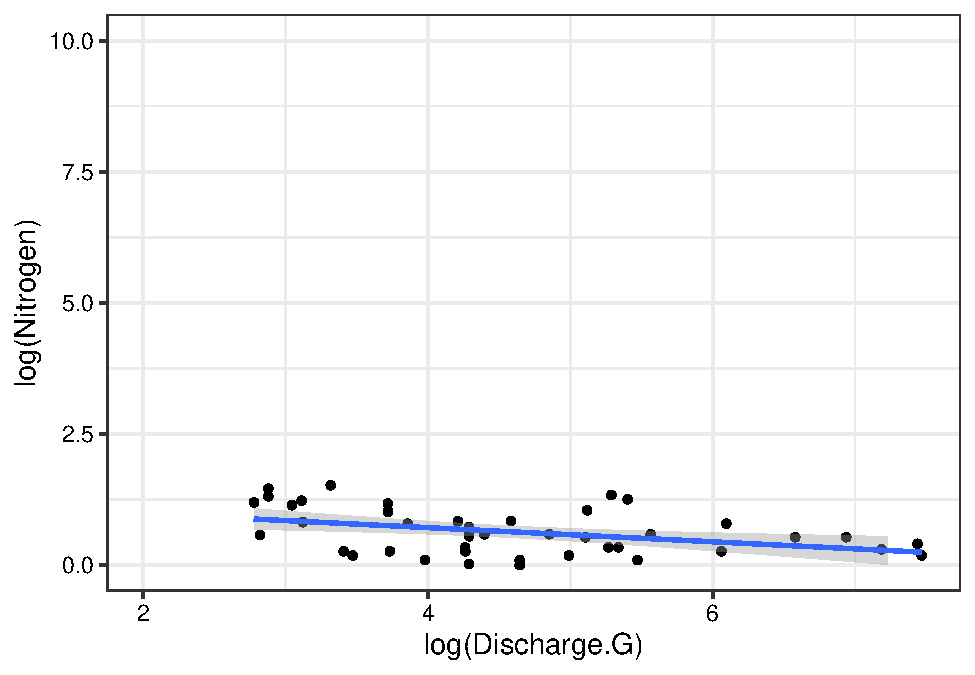
\includegraphics{Project_DataAnalysis_files/figure-latex/unnamed-chunk-5-1.pdf}

\begin{Shaded}
\begin{Highlighting}[]
\CommentTok{### histogram shows data is not very rightly skewed }

\KeywordTok{qqnorm}\NormalTok{(EC_Flow.Nutrients_Wide}\OperatorTok{$}\NormalTok{Mixed_N); }\KeywordTok{qqline}\NormalTok{(EC_Flow.Nutrients_Wide}\OperatorTok{$}\NormalTok{Mixed_N)}
\end{Highlighting}
\end{Shaded}

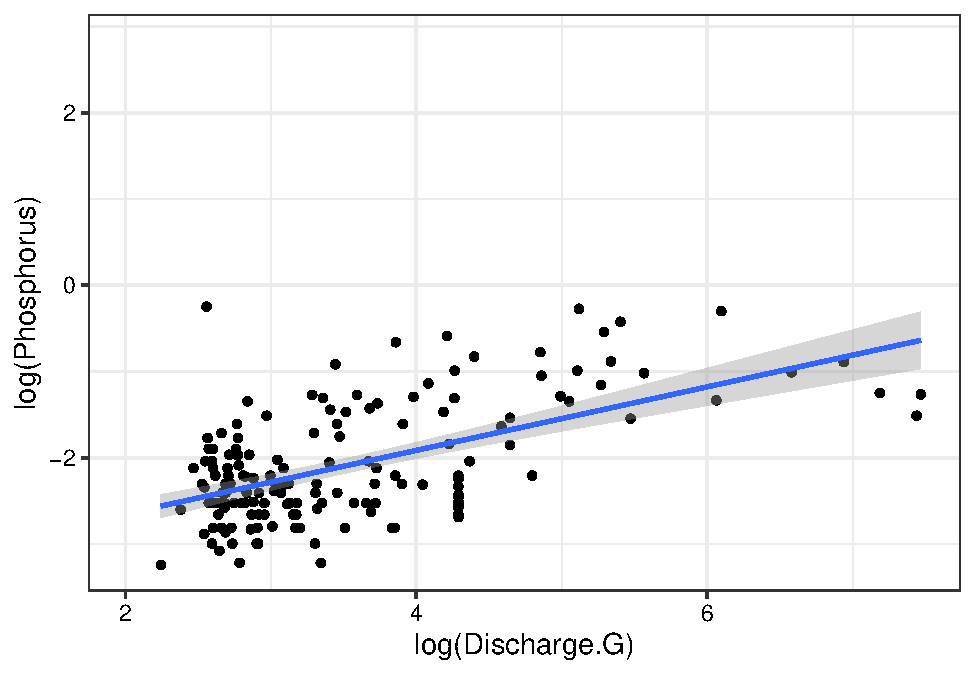
\includegraphics{Project_DataAnalysis_files/figure-latex/unnamed-chunk-5-2.pdf}

\begin{Shaded}
\begin{Highlighting}[]
\CommentTok{## some samples are higher than normal and some are lower}

\NormalTok{N.onesample <-}\StringTok{ }\KeywordTok{t.test}\NormalTok{(EC_Flow.Nutrients_Wide}\OperatorTok{$}\NormalTok{Mixed_N, }\DataTypeTok{mu =} \DecValTok{10}\NormalTok{, }\DataTypeTok{alternative =} \StringTok{"greater"}\NormalTok{)}
\NormalTok{N.onesample}
\end{Highlighting}
\end{Shaded}

\begin{verbatim}
## 
##  One Sample t-test
## 
## data:  EC_Flow.Nutrients_Wide$Mixed_N
## t = 3.5158, df = 139, p-value = 0.0002962
## alternative hypothesis: true mean is greater than 10
## 95 percent confidence interval:
##  13.31248      Inf
## sample estimates:
## mean of x 
##  16.26161
\end{verbatim}

\begin{Shaded}
\begin{Highlighting}[]
\CommentTok{# Null hypothesis is that mean = 10, alternative is mean is less than 10}
\CommentTok{# p value >0.05 so we can reject the null the mean =10}

\CommentTok{# plot }

\NormalTok{N.plot <-}\StringTok{ }\KeywordTok{ggplot}\NormalTok{(EC_Flow.Nutrients_Wide, }\KeywordTok{aes}\NormalTok{(}\DataTypeTok{x =}\NormalTok{ Mixed_N)) }\OperatorTok{+}
\StringTok{  }\CommentTok{#geom_density(stat = "count", fill = "gray") + #<-shows count so it's more jagged}
\StringTok{  }\KeywordTok{geom_density}\NormalTok{(}\DataTypeTok{fill =} \StringTok{"gray"}\NormalTok{) }\OperatorTok{+}
\StringTok{  }\KeywordTok{geom_vline}\NormalTok{(}\DataTypeTok{xintercept =} \DecValTok{10}\NormalTok{, }\DataTypeTok{color =} \StringTok{"#238b45"}\NormalTok{, }\DataTypeTok{lty =} \DecValTok{2}\NormalTok{, }\DataTypeTok{size =} \FloatTok{0.9}\NormalTok{) }\OperatorTok{+}
\StringTok{  }\KeywordTok{scale_x_continuous}\NormalTok{(}\DataTypeTok{expand =} \KeywordTok{c}\NormalTok{(}\DecValTok{0}\NormalTok{, }\DecValTok{0}\NormalTok{)) }\OperatorTok{+}\StringTok{ }\KeywordTok{scale_y_continuous}\NormalTok{(}\DataTypeTok{expand =} \KeywordTok{c}\NormalTok{(}\DecValTok{0}\NormalTok{, }\DecValTok{0}\NormalTok{))}
\KeywordTok{print}\NormalTok{(N.plot)}
\end{Highlighting}
\end{Shaded}

\begin{verbatim}
## Warning: Removed 5490 rows containing non-finite values (stat_density).
\end{verbatim}

\includegraphics{Project_DataAnalysis_files/figure-latex/unnamed-chunk-5-3.pdf}
\#\#\#\#\# Nitrogen Results \textgreater{} Nitrogen measurments in
ellerbe creek were not significantly greater than 10 mg/L, the Maximum
Contaminent Level for Nitrogen in drinking water (one sample t-test; t=
3.515, df = 139, p \textless{} 0.001)

\hypertarget{phosphorus}{%
\subsubsection{Phosphorus}\label{phosphorus}}

\begin{Shaded}
\begin{Highlighting}[]
\KeywordTok{summary}\NormalTok{(EC_Flow.Nutrients_Wide}\OperatorTok{$}\NormalTok{TP)}
\end{Highlighting}
\end{Shaded}

\begin{verbatim}
##    Min. 1st Qu.  Median    Mean 3rd Qu.    Max.    NA's 
##   0.039   0.087   0.159   1.577   0.660  34.500    5387
\end{verbatim}

\begin{Shaded}
\begin{Highlighting}[]
\CommentTok{# Evaluate assumption of normal distribution }
\KeywordTok{shapiro.test}\NormalTok{((EC_Flow.Nutrients_Wide}\OperatorTok{$}\NormalTok{TP))}
\end{Highlighting}
\end{Shaded}

\begin{verbatim}
## 
##  Shapiro-Wilk normality test
## 
## data:  (EC_Flow.Nutrients_Wide$TP)
## W = 0.47359, p-value < 2.2e-16
\end{verbatim}

\begin{Shaded}
\begin{Highlighting}[]
\CommentTok{### shapiro wilke test the null hypothesis is that the data are a normal distribution }
\CommentTok{### p value <0.05 shows we reject null and data is not normally distributed}
\CommentTok{######## "not well approximated by a normal distribution"}

\KeywordTok{ggplot}\NormalTok{(EC_Flow.Nutrients_Wide, }\KeywordTok{aes}\NormalTok{(}\DataTypeTok{x =}\NormalTok{ TP)) }\OperatorTok{+}
\StringTok{  }\KeywordTok{geom_histogram}\NormalTok{(}\DataTypeTok{binwidth =} \DecValTok{1}\NormalTok{) }
\end{Highlighting}
\end{Shaded}

\begin{verbatim}
## Warning: Removed 5387 rows containing non-finite values (stat_bin).
\end{verbatim}

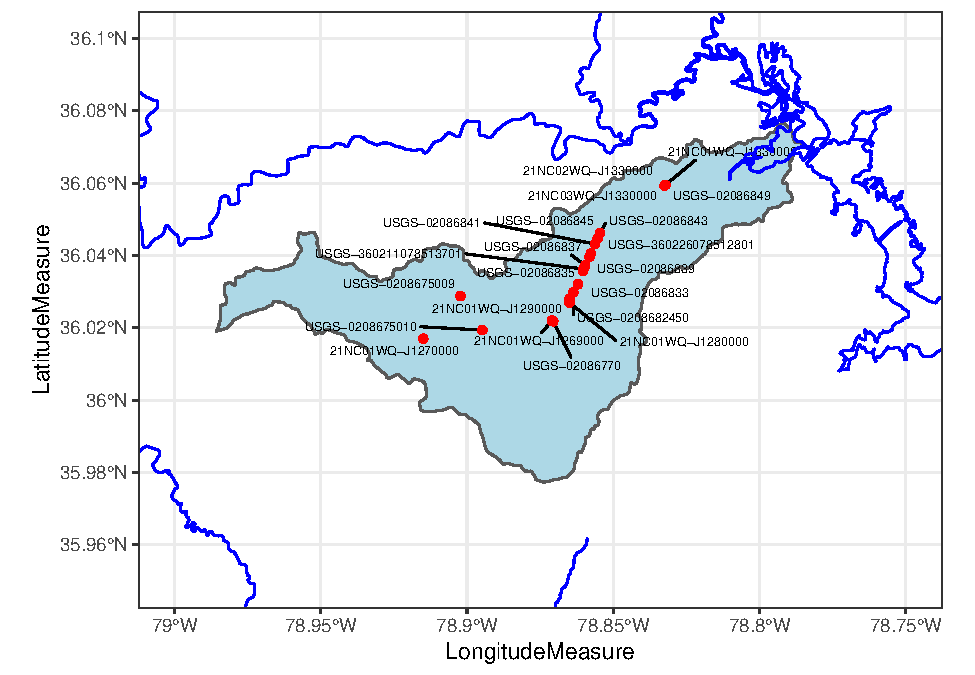
\includegraphics{Project_DataAnalysis_files/figure-latex/unnamed-chunk-6-1.pdf}

\begin{Shaded}
\begin{Highlighting}[]
\CommentTok{### histogram shows data is not very rightly skewed }

\KeywordTok{qqnorm}\NormalTok{(EC_Flow.Nutrients_Wide}\OperatorTok{$}\NormalTok{TP); }\KeywordTok{qqline}\NormalTok{(EC_Flow.Nutrients_Wide}\OperatorTok{$}\NormalTok{TP)}
\end{Highlighting}
\end{Shaded}

\includegraphics{Project_DataAnalysis_files/figure-latex/unnamed-chunk-6-2.pdf}

\begin{Shaded}
\begin{Highlighting}[]
\CommentTok{## samples are higher than normal distribution}

\NormalTok{P.onesample <-}\StringTok{ }\KeywordTok{t.test}\NormalTok{(EC_Flow.Nutrients_Wide}\OperatorTok{$}\NormalTok{TP, }\DataTypeTok{mu =} \DecValTok{1}\NormalTok{, }\DataTypeTok{alternative =} \StringTok{"greater"}\NormalTok{)}
\NormalTok{P.onesample}
\end{Highlighting}
\end{Shaded}

\begin{verbatim}
## 
##  One Sample t-test
## 
## data:  EC_Flow.Nutrients_Wide$TP
## t = 2.5264, df = 242, p-value = 0.006081
## alternative hypothesis: true mean is greater than 1
## 95 percent confidence interval:
##  1.199743      Inf
## sample estimates:
## mean of x 
##  1.576553
\end{verbatim}

\begin{Shaded}
\begin{Highlighting}[]
\CommentTok{# Null hypothesis is that mean = 1, alternative is mean is less than 1}
\CommentTok{# p value <0.05 so we can reject the null the mean = 1}

\CommentTok{# plot }

\NormalTok{P.plot <-}\StringTok{ }\KeywordTok{ggplot}\NormalTok{(EC_Flow.Nutrients_Wide, }\KeywordTok{aes}\NormalTok{(}\DataTypeTok{x =}\NormalTok{ TP)) }\OperatorTok{+}
\StringTok{  }\CommentTok{#geom_density(stat = "count", fill = "gray") + #<-shows count so it's more jagged}
\StringTok{  }\KeywordTok{geom_density}\NormalTok{(}\DataTypeTok{fill =} \StringTok{"gray"}\NormalTok{) }\OperatorTok{+}
\StringTok{  }\KeywordTok{geom_vline}\NormalTok{(}\DataTypeTok{xintercept =} \DecValTok{1}\NormalTok{, }\DataTypeTok{color =} \StringTok{"#238b45"}\NormalTok{, }\DataTypeTok{lty =} \DecValTok{2}\NormalTok{, }\DataTypeTok{size =} \FloatTok{0.9}\NormalTok{) }\OperatorTok{+}
\StringTok{  }\KeywordTok{scale_x_continuous}\NormalTok{(}\DataTypeTok{expand =} \KeywordTok{c}\NormalTok{(}\DecValTok{0}\NormalTok{, }\DecValTok{0}\NormalTok{)) }\OperatorTok{+}\StringTok{ }\KeywordTok{scale_y_continuous}\NormalTok{(}\DataTypeTok{expand =} \KeywordTok{c}\NormalTok{(}\DecValTok{0}\NormalTok{, }\DecValTok{0}\NormalTok{))}
\KeywordTok{print}\NormalTok{(N.plot)}
\end{Highlighting}
\end{Shaded}

\begin{verbatim}
## Warning: Removed 5490 rows containing non-finite values (stat_density).
\end{verbatim}

\includegraphics{Project_DataAnalysis_files/figure-latex/unnamed-chunk-6-3.pdf}
\#\#\#\#\# Phosphorus Results \textgreater{} Phosphorus measurments in
ellerbe creek were significantly greater than 1 mg/L, the Maximum
Contaminent Level for phosphorus in water (one sample t-test; t= 2.5264,
df = 242, p = 0.006)

\#Two Sample t-test (Upstream vs.~Downstream) \#\#\# Nitrogen

\begin{Shaded}
\begin{Highlighting}[]
\KeywordTok{shapiro.test}\NormalTok{(Club.Gorman_Flow.Nutrients_Wide}\OperatorTok{$}\NormalTok{Mixed_N[Club.Gorman_Flow.Nutrients_Wide}\OperatorTok{$}\NormalTok{Location }\OperatorTok{==}\StringTok{ "Upstream"}\NormalTok{])}
\end{Highlighting}
\end{Shaded}

\begin{verbatim}
## 
##  Shapiro-Wilk normality test
## 
## data:  Club.Gorman_Flow.Nutrients_Wide$Mixed_N[Club.Gorman_Flow.Nutrients_Wide$Location ==     "Upstream"]
## W = 0.93963, p-value = 0.06625
\end{verbatim}

\begin{Shaded}
\begin{Highlighting}[]
\KeywordTok{shapiro.test}\NormalTok{(Club.Gorman_Flow.Nutrients_Wide}\OperatorTok{$}\NormalTok{Mixed_N[Club.Gorman_Flow.Nutrients_Wide}\OperatorTok{$}\NormalTok{Location }\OperatorTok{==}\StringTok{ "Downstream"}\NormalTok{])}
\end{Highlighting}
\end{Shaded}

\begin{verbatim}
## 
##  Shapiro-Wilk normality test
## 
## data:  Club.Gorman_Flow.Nutrients_Wide$Mixed_N[Club.Gorman_Flow.Nutrients_Wide$Location ==     "Downstream"]
## W = 0.87157, p-value = 1.642e-07
\end{verbatim}

\begin{Shaded}
\begin{Highlighting}[]
\KeywordTok{var.test}\NormalTok{(Club.Gorman_Flow.Nutrients_Wide}\OperatorTok{$}\NormalTok{Mixed_N }\OperatorTok{~}\StringTok{ }\NormalTok{Club.Gorman_Flow.Nutrients_Wide}\OperatorTok{$}\NormalTok{Location)}
\end{Highlighting}
\end{Shaded}

\begin{verbatim}
## 
##  F test to compare two variances
## 
## data:  Club.Gorman_Flow.Nutrients_Wide$Mixed_N by Club.Gorman_Flow.Nutrients_Wide$Location
## F = 1862.5, num df = 93, denom df = 32, p-value < 2.2e-16
## alternative hypothesis: true ratio of variances is not equal to 1
## 95 percent confidence interval:
##  1005.094 3181.440
## sample estimates:
## ratio of variances 
##           1862.531
\end{verbatim}

\begin{Shaded}
\begin{Highlighting}[]
\CommentTok{### "var.test" test variance }
\CommentTok{### asks are the variances eqaul - what is the diff between variances }
\CommentTok{### results: variances are significantly different }
\CommentTok{### results: violate assumption of normality and equal variance}

\KeywordTok{ggplot}\NormalTok{(Club.Gorman_Flow.Nutrients_Wide, }\KeywordTok{aes}\NormalTok{(}\DataTypeTok{x =}\NormalTok{ Mixed_N, }\DataTypeTok{color =}\NormalTok{ Location)) }\OperatorTok{+}
\StringTok{  }\KeywordTok{geom_freqpoly}\NormalTok{()}
\end{Highlighting}
\end{Shaded}

\begin{verbatim}
## `stat_bin()` using `bins = 30`. Pick better value with `binwidth`.
\end{verbatim}

\begin{verbatim}
## Warning: Removed 9854 rows containing non-finite values (stat_bin).
\end{verbatim}

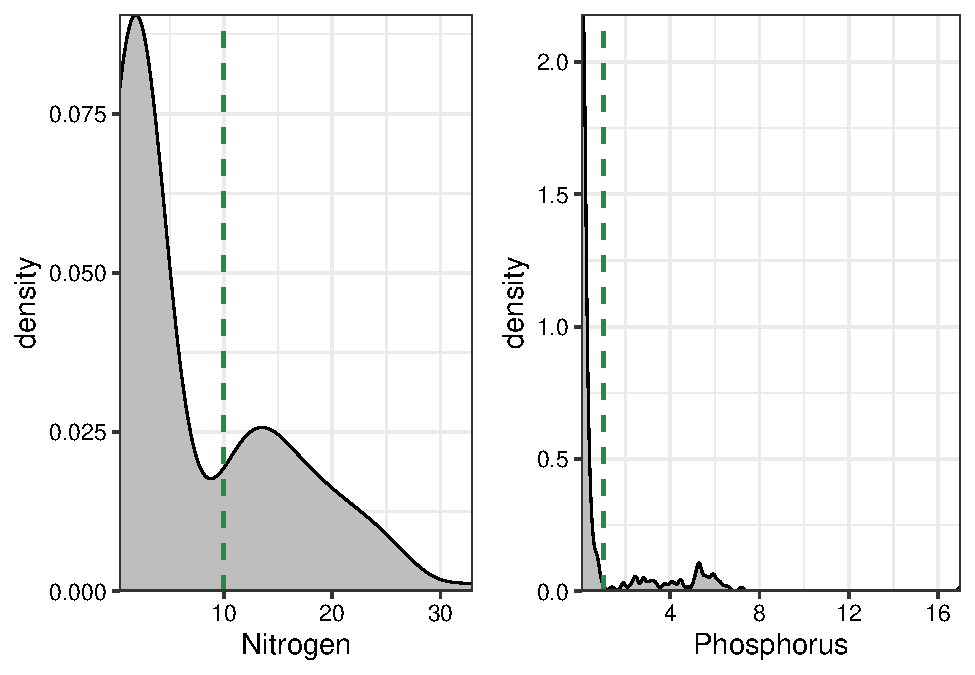
\includegraphics{Project_DataAnalysis_files/figure-latex/unnamed-chunk-7-1.pdf}

\begin{Shaded}
\begin{Highlighting}[]
\NormalTok{N.twosample <-}\StringTok{ }\KeywordTok{t.test}\NormalTok{(Club.Gorman_Flow.Nutrients_Wide}\OperatorTok{$}\NormalTok{Mixed_N }\OperatorTok{~}\StringTok{ }\NormalTok{Club.Gorman_Flow.Nutrients_Wide}\OperatorTok{$}\NormalTok{Location)}
\NormalTok{N.twosample}
\end{Highlighting}
\end{Shaded}

\begin{verbatim}
## 
##  Welch Two Sample t-test
## 
## data:  Club.Gorman_Flow.Nutrients_Wide$Mixed_N by Club.Gorman_Flow.Nutrients_Wide$Location
## t = 9.7326, df = 93.284, p-value = 7.313e-16
## alternative hypothesis: true difference in means is not equal to 0
## 95 percent confidence interval:
##  17.85949 27.01521
## sample estimates:
## mean in group Downstream   mean in group Upstream 
##                23.578564                 1.141212
\end{verbatim}

\hypertarget{phosphorus-1}{%
\subsubsection{Phosphorus}\label{phosphorus-1}}

\begin{Shaded}
\begin{Highlighting}[]
\KeywordTok{shapiro.test}\NormalTok{(Club.Gorman_Flow.Nutrients_Wide}\OperatorTok{$}\NormalTok{TP[Club.Gorman_Flow.Nutrients_Wide}\OperatorTok{$}\NormalTok{Location }\OperatorTok{==}\StringTok{ "Upstream"}\NormalTok{])}
\end{Highlighting}
\end{Shaded}

\begin{verbatim}
## 
##  Shapiro-Wilk normality test
## 
## data:  Club.Gorman_Flow.Nutrients_Wide$TP[Club.Gorman_Flow.Nutrients_Wide$Location ==     "Upstream"]
## W = 0.88509, p-value = 0.001368
\end{verbatim}

\begin{Shaded}
\begin{Highlighting}[]
\KeywordTok{shapiro.test}\NormalTok{(Club.Gorman_Flow.Nutrients_Wide}\OperatorTok{$}\NormalTok{TP[Club.Gorman_Flow.Nutrients_Wide}\OperatorTok{$}\NormalTok{Location }\OperatorTok{==}\StringTok{ "Downstream"}\NormalTok{])}
\end{Highlighting}
\end{Shaded}

\begin{verbatim}
## 
##  Shapiro-Wilk normality test
## 
## data:  Club.Gorman_Flow.Nutrients_Wide$TP[Club.Gorman_Flow.Nutrients_Wide$Location ==     "Downstream"]
## W = 0.52423, p-value < 2.2e-16
\end{verbatim}

\begin{Shaded}
\begin{Highlighting}[]
\KeywordTok{var.test}\NormalTok{(Club.Gorman_Flow.Nutrients_Wide}\OperatorTok{$}\NormalTok{TP }\OperatorTok{~}\StringTok{ }\NormalTok{Club.Gorman_Flow.Nutrients_Wide}\OperatorTok{$}\NormalTok{Location)}
\end{Highlighting}
\end{Shaded}

\begin{verbatim}
## 
##  F test to compare two variances
## 
## data:  Club.Gorman_Flow.Nutrients_Wide$TP by Club.Gorman_Flow.Nutrients_Wide$Location
## F = 524.21, num df = 196, denom df = 35, p-value < 2.2e-16
## alternative hypothesis: true ratio of variances is not equal to 1
## 95 percent confidence interval:
##  298.9121 837.7713
## sample estimates:
## ratio of variances 
##           524.2082
\end{verbatim}

\begin{Shaded}
\begin{Highlighting}[]
\CommentTok{### "var.test" test variance }
\CommentTok{### asks are the variances eqaul - what is the diff between variances }
\CommentTok{### results: variances are significantly different }
\CommentTok{### results: violate assumption of normality and equal variance}

\KeywordTok{ggplot}\NormalTok{(Club.Gorman_Flow.Nutrients_Wide, }\KeywordTok{aes}\NormalTok{(}\DataTypeTok{x =}\NormalTok{ TP, }\DataTypeTok{color =}\NormalTok{ Location)) }\OperatorTok{+}
\StringTok{  }\KeywordTok{geom_freqpoly}\NormalTok{()}
\end{Highlighting}
\end{Shaded}

\begin{verbatim}
## `stat_bin()` using `bins = 30`. Pick better value with `binwidth`.
\end{verbatim}

\begin{verbatim}
## Warning: Removed 9748 rows containing non-finite values (stat_bin).
\end{verbatim}

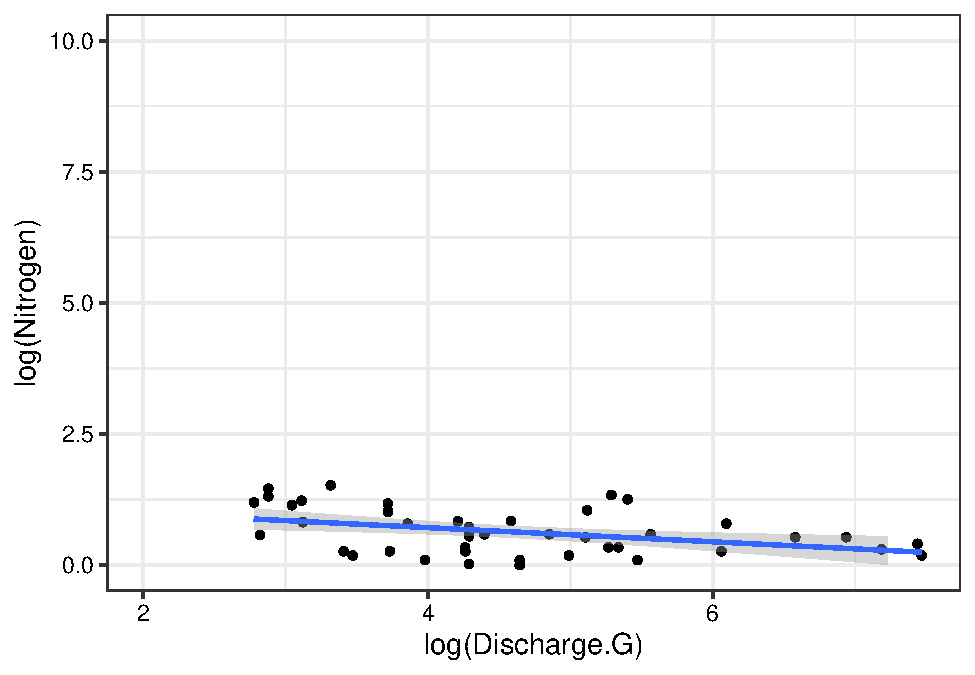
\includegraphics{Project_DataAnalysis_files/figure-latex/unnamed-chunk-8-1.pdf}

\begin{Shaded}
\begin{Highlighting}[]
\NormalTok{P.twosample <-}\StringTok{ }\KeywordTok{t.test}\NormalTok{(Club.Gorman_Flow.Nutrients_Wide}\OperatorTok{$}\NormalTok{TP }\OperatorTok{~}\StringTok{ }\NormalTok{Club.Gorman_Flow.Nutrients_Wide}\OperatorTok{$}\NormalTok{Location)}
\NormalTok{P.twosample}
\end{Highlighting}
\end{Shaded}

\begin{verbatim}
## 
##  Welch Two Sample t-test
## 
## data:  Club.Gorman_Flow.Nutrients_Wide$TP by Club.Gorman_Flow.Nutrients_Wide$Location
## t = 6.0272, df = 199.99, p-value = 7.906e-09
## alternative hypothesis: true difference in means is not equal to 0
## 95 percent confidence interval:
##  1.127322 2.223637
## sample estimates:
## mean in group Downstream   mean in group Upstream 
##                 1.899354                 0.223875
\end{verbatim}

\hypertarget{wilcox-test-dont-assume-normality}{%
\section{Wilcox Test (Don't Assume
Normality)}\label{wilcox-test-dont-assume-normality}}

\hypertarget{nitrogen-1}{%
\subsubsection{Nitrogen}\label{nitrogen-1}}

\begin{Shaded}
\begin{Highlighting}[]
\NormalTok{N.onesample.wilcox <-}\StringTok{ }\KeywordTok{wilcox.test}\NormalTok{(Club.Gorman_Flow.Nutrients_Wide}\OperatorTok{$}\NormalTok{Mixed_N, }\DataTypeTok{mu =} \DecValTok{10}\NormalTok{, }\DataTypeTok{alternative =} \StringTok{"greater"}\NormalTok{)}
\NormalTok{N.onesample.wilcox}
\end{Highlighting}
\end{Shaded}

\begin{verbatim}
## 
##  Wilcoxon signed rank test with continuity correction
## 
## data:  Club.Gorman_Flow.Nutrients_Wide$Mixed_N
## V = 4687, p-value = 0.04743
## alternative hypothesis: true location is greater than 10
\end{verbatim}

\begin{Shaded}
\begin{Highlighting}[]
\NormalTok{N.twosample.wilcox <-}\StringTok{ }\KeywordTok{wilcox.test}\NormalTok{(Club.Gorman_Flow.Nutrients_Wide}\OperatorTok{$}\NormalTok{Mixed_N }\OperatorTok{~}\StringTok{ }\NormalTok{Club.Gorman_Flow.Nutrients_Wide}\OperatorTok{$}\NormalTok{Location)}
\NormalTok{N.twosample.wilcox}
\end{Highlighting}
\end{Shaded}

\begin{verbatim}
## 
##  Wilcoxon rank sum test with continuity correction
## 
## data:  Club.Gorman_Flow.Nutrients_Wide$Mixed_N by Club.Gorman_Flow.Nutrients_Wide$Location
## W = 2988, p-value = 2.832e-15
## alternative hypothesis: true location shift is not equal to 0
\end{verbatim}

\hypertarget{phosphorus-2}{%
\subsubsection{Phosphorus}\label{phosphorus-2}}

\begin{Shaded}
\begin{Highlighting}[]
\NormalTok{P.onesample.wilcox <-}\StringTok{ }\KeywordTok{wilcox.test}\NormalTok{(Club.Gorman_Flow.Nutrients_Wide}\OperatorTok{$}\NormalTok{TP, }\DataTypeTok{mu =} \DecValTok{1}\NormalTok{, }\DataTypeTok{alternative =} \StringTok{"greater"}\NormalTok{)}
\NormalTok{P.onesample.wilcox}
\end{Highlighting}
\end{Shaded}

\begin{verbatim}
## 
##  Wilcoxon signed rank test with continuity correction
## 
## data:  Club.Gorman_Flow.Nutrients_Wide$TP
## V = 10454, p-value = 0.999
## alternative hypothesis: true location is greater than 1
\end{verbatim}

\begin{Shaded}
\begin{Highlighting}[]
\NormalTok{P.twosample.wilcox <-}\StringTok{ }\KeywordTok{wilcox.test}\NormalTok{(Club.Gorman_Flow.Nutrients_Wide}\OperatorTok{$}\NormalTok{TP }\OperatorTok{~}\StringTok{ }\NormalTok{Club.Gorman_Flow.Nutrients_Wide}\OperatorTok{$}\NormalTok{Location)}
\NormalTok{P.twosample.wilcox}
\end{Highlighting}
\end{Shaded}

\begin{verbatim}
## 
##  Wilcoxon rank sum test with continuity correction
## 
## data:  Club.Gorman_Flow.Nutrients_Wide$TP by Club.Gorman_Flow.Nutrients_Wide$Location
## W = 4136, p-value = 0.1128
## alternative hypothesis: true location shift is not equal to 0
\end{verbatim}

\hypertarget{simple-linear-regression}{%
\section{Simple Linear Regression}\label{simple-linear-regression}}

\begin{quote}
Is flow a significant predictor of nutrient levels? continuous response
(N or P) continuous predictor (discharge)
\end{quote}

\#\#\#Nitrogen

\begin{Shaded}
\begin{Highlighting}[]
\NormalTok{NitrogenClub.regression <-}\KeywordTok{lm}\NormalTok{(}\DataTypeTok{data =}\NormalTok{ EC_Flow.Nutrients_Wide, Mixed_N }\OperatorTok{~}\StringTok{ }\NormalTok{Discharge.C)}
\KeywordTok{summary}\NormalTok{(NitrogenClub.regression)}
\end{Highlighting}
\end{Shaded}

\begin{verbatim}
## 
## Call:
## lm(formula = Mixed_N ~ Discharge.C, data = EC_Flow.Nutrients_Wide)
## 
## Residuals:
##      Min       1Q   Median       3Q      Max 
## -1.38192 -0.75099 -0.09027  0.47413  2.81925 
## 
## Coefficients:
##               Estimate Std. Error t value Pr(>|t|)    
## (Intercept)  1.7519765  0.1382810  12.670   <2e-16 ***
## Discharge.C -0.0006604  0.0011685  -0.565    0.574    
## ---
## Signif. codes:  0 '***' 0.001 '**' 0.01 '*' 0.05 '.' 0.1 ' ' 1
## 
## Residual standard error: 1.002 on 62 degrees of freedom
##   (5566 observations deleted due to missingness)
## Multiple R-squared:  0.005126,   Adjusted R-squared:  -0.01092 
## F-statistic: 0.3195 on 1 and 62 DF,  p-value: 0.574
\end{verbatim}

\begin{Shaded}
\begin{Highlighting}[]
\CommentTok{## adj R squared says 1 % of variance is explained by depth }

\KeywordTok{cor.test}\NormalTok{(EC_Flow.Nutrients_Wide}\OperatorTok{$}\NormalTok{Mixed_N, EC_Flow.Nutrients_Wide}\OperatorTok{$}\NormalTok{Discharge.C)}
\end{Highlighting}
\end{Shaded}

\begin{verbatim}
## 
##  Pearson's product-moment correlation
## 
## data:  EC_Flow.Nutrients_Wide$Mixed_N and EC_Flow.Nutrients_Wide$Discharge.C
## t = -0.56521, df = 62, p-value = 0.574
## alternative hypothesis: true correlation is not equal to 0
## 95 percent confidence interval:
##  -0.3119172  0.1773328
## sample estimates:
##         cor 
## -0.07159742
\end{verbatim}

\begin{Shaded}
\begin{Highlighting}[]
\NormalTok{NitrogenGorman.regression <-}\KeywordTok{lm}\NormalTok{(}\DataTypeTok{data =}\NormalTok{ EC_Flow.Nutrients_Wide, Mixed_N }\OperatorTok{~}\StringTok{ }\NormalTok{Discharge.G)}
\KeywordTok{summary}\NormalTok{(NitrogenGorman.regression)}
\end{Highlighting}
\end{Shaded}

\begin{verbatim}
## 
## Call:
## lm(formula = Mixed_N ~ Discharge.G, data = EC_Flow.Nutrients_Wide)
## 
## Residuals:
##     Min      1Q  Median      3Q     Max 
## -1.3766 -0.7452 -0.1024  0.4735  2.8263 
## 
## Coefficients:
##               Estimate Std. Error t value Pr(>|t|)    
## (Intercept)  1.7481842  0.1405379  12.439   <2e-16 ***
## Discharge.G -0.0001626  0.0003524  -0.461    0.646    
## ---
## Signif. codes:  0 '***' 0.001 '**' 0.01 '*' 0.05 '.' 0.1 ' ' 1
## 
## Residual standard error: 1.003 on 62 degrees of freedom
##   (5566 observations deleted due to missingness)
## Multiple R-squared:  0.003423,   Adjusted R-squared:  -0.01265 
## F-statistic: 0.2129 on 1 and 62 DF,  p-value: 0.6461
\end{verbatim}

\begin{Shaded}
\begin{Highlighting}[]
\CommentTok{## adj R squared says 1 % of variance is explained by depth }

\KeywordTok{cor.test}\NormalTok{(EC_Flow.Nutrients_Wide}\OperatorTok{$}\NormalTok{Mixed_N, EC_Flow.Nutrients_Wide}\OperatorTok{$}\NormalTok{Discharge.G)}
\end{Highlighting}
\end{Shaded}

\begin{verbatim}
## 
##  Pearson's product-moment correlation
## 
## data:  EC_Flow.Nutrients_Wide$Mixed_N and EC_Flow.Nutrients_Wide$Discharge.G
## t = -0.46144, df = 62, p-value = 0.6461
## alternative hypothesis: true correlation is not equal to 0
## 95 percent confidence interval:
##  -0.2999978  0.1900395
## sample estimates:
##         cor 
## -0.05850268
\end{verbatim}

\#\#\#Phosphorus

\begin{Shaded}
\begin{Highlighting}[]
\NormalTok{PhosphorusClub.regression <-}\KeywordTok{lm}\NormalTok{(}\DataTypeTok{data =}\NormalTok{ EC_Flow.Nutrients_Wide, TP }\OperatorTok{~}\StringTok{ }\NormalTok{Discharge.C)}
\KeywordTok{summary}\NormalTok{(PhosphorusClub.regression)}
\end{Highlighting}
\end{Shaded}

\begin{verbatim}
## 
## Call:
## lm(formula = TP ~ Discharge.C, data = EC_Flow.Nutrients_Wide)
## 
## Residuals:
##      Min       1Q   Median       3Q      Max 
## -0.30568 -0.07026 -0.04760  0.02954  0.59927 
## 
## Coefficients:
##              Estimate Std. Error t value Pr(>|t|)    
## (Intercept) 0.1450530  0.0106823  13.579  < 2e-16 ***
## Discharge.C 0.0005484  0.0001417   3.872 0.000158 ***
## ---
## Signif. codes:  0 '***' 0.001 '**' 0.01 '*' 0.05 '.' 0.1 ' ' 1
## 
## Residual standard error: 0.1286 on 157 degrees of freedom
##   (5471 observations deleted due to missingness)
## Multiple R-squared:  0.08715,    Adjusted R-squared:  0.08134 
## F-statistic: 14.99 on 1 and 157 DF,  p-value: 0.0001583
\end{verbatim}

\begin{Shaded}
\begin{Highlighting}[]
\CommentTok{## adj R squared says 8 % of variance is explained by depth }
\CommentTok{## significant relationship p < 0.001}

\KeywordTok{cor.test}\NormalTok{(EC_Flow.Nutrients_Wide}\OperatorTok{$}\NormalTok{TP, EC_Flow.Nutrients_Wide}\OperatorTok{$}\NormalTok{Discharge.C)}
\end{Highlighting}
\end{Shaded}

\begin{verbatim}
## 
##  Pearson's product-moment correlation
## 
## data:  EC_Flow.Nutrients_Wide$TP and EC_Flow.Nutrients_Wide$Discharge.C
## t = 3.8716, df = 157, p-value = 0.0001583
## alternative hypothesis: true correlation is not equal to 0
## 95 percent confidence interval:
##  0.1462907 0.4310563
## sample estimates:
##       cor 
## 0.2952159
\end{verbatim}

\begin{Shaded}
\begin{Highlighting}[]
\NormalTok{PhosphorusGorman.regression <-}\KeywordTok{lm}\NormalTok{(}\DataTypeTok{data =}\NormalTok{ EC_Flow.Nutrients_Wide, TP }\OperatorTok{~}\StringTok{ }\NormalTok{Discharge.G)}
\KeywordTok{summary}\NormalTok{(PhosphorusGorman.regression)}
\end{Highlighting}
\end{Shaded}

\begin{verbatim}
## 
## Call:
## lm(formula = TP ~ Discharge.G, data = EC_Flow.Nutrients_Wide)
## 
## Residuals:
##      Min       1Q   Median       3Q      Max 
## -0.24129 -0.07216 -0.04873  0.02568  0.63304 
## 
## Coefficients:
##              Estimate Std. Error t value Pr(>|t|)    
## (Intercept) 1.446e-01  1.117e-02  12.939  < 2e-16 ***
## Discharge.G 1.863e-04  4.457e-05   4.181 4.75e-05 ***
## ---
## Signif. codes:  0 '***' 0.001 '**' 0.01 '*' 0.05 '.' 0.1 ' ' 1
## 
## Residual standard error: 0.1343 on 162 degrees of freedom
##   (5466 observations deleted due to missingness)
## Multiple R-squared:  0.09738,    Adjusted R-squared:  0.0918 
## F-statistic: 17.48 on 1 and 162 DF,  p-value: 4.749e-05
\end{verbatim}

\begin{Shaded}
\begin{Highlighting}[]
\CommentTok{## adj R squared says 9 % of variance is explained by depth}
\CommentTok{## significant relationship p < 0.001}

\KeywordTok{cor.test}\NormalTok{(EC_Flow.Nutrients_Wide}\OperatorTok{$}\NormalTok{TP, EC_Flow.Nutrients_Wide}\OperatorTok{$}\NormalTok{Discharge.G)}
\end{Highlighting}
\end{Shaded}

\begin{verbatim}
## 
##  Pearson's product-moment correlation
## 
## data:  EC_Flow.Nutrients_Wide$TP and EC_Flow.Nutrients_Wide$Discharge.G
## t = 4.1805, df = 162, p-value = 4.749e-05
## alternative hypothesis: true correlation is not equal to 0
## 95 percent confidence interval:
##  0.1667759 0.4440642
## sample estimates:
##       cor 
## 0.3120502
\end{verbatim}

\hypertarget{plot-regression}{%
\section{Plot Regression}\label{plot-regression}}

\hypertarget{nitrogen-2}{%
\subsubsection{Nitrogen}\label{nitrogen-2}}

\begin{Shaded}
\begin{Highlighting}[]
\NormalTok{Nitrogen_Discharge <-}\StringTok{ }
\StringTok{  }\KeywordTok{ggplot}\NormalTok{(EC_Flow.Nutrients_Wide, }\KeywordTok{aes}\NormalTok{ (}\DataTypeTok{x=}\NormalTok{Discharge.G, }\DataTypeTok{y =}\NormalTok{ Mixed_N))}\OperatorTok{+}
\StringTok{  }\KeywordTok{geom_point}\NormalTok{()}\OperatorTok{+}
\StringTok{  }\KeywordTok{geom_smooth}\NormalTok{(}\DataTypeTok{method=}\NormalTok{lm)}\OperatorTok{+}
\StringTok{  }\KeywordTok{ylim}\NormalTok{(}\DecValTok{0}\NormalTok{,}\DecValTok{10}\NormalTok{)}
\KeywordTok{print}\NormalTok{(Nitrogen_Discharge)}
\end{Highlighting}
\end{Shaded}

\begin{verbatim}
## Warning: Removed 5566 rows containing non-finite values (stat_smooth).
\end{verbatim}

\begin{verbatim}
## Warning: Removed 5566 rows containing missing values (geom_point).
\end{verbatim}

\includegraphics{Project_DataAnalysis_files/figure-latex/unnamed-chunk-13-1.pdf}

\begin{Shaded}
\begin{Highlighting}[]
\CommentTok{#log discharge }
\NormalTok{Nitrogen_logDischarge <-}\StringTok{ }
\StringTok{  }\KeywordTok{ggplot}\NormalTok{(EC_Flow.Nutrients_Wide, }\KeywordTok{aes}\NormalTok{ (}\DataTypeTok{x=}\KeywordTok{log}\NormalTok{(Discharge.G), }\DataTypeTok{y =}\NormalTok{ Mixed_N))}\OperatorTok{+}
\StringTok{  }\KeywordTok{geom_point}\NormalTok{()}\OperatorTok{+}
\StringTok{  }\KeywordTok{geom_smooth}\NormalTok{(}\DataTypeTok{method=}\NormalTok{lm)}\OperatorTok{+}
\StringTok{  }\KeywordTok{ylim}\NormalTok{(}\DecValTok{0}\NormalTok{,}\DecValTok{10}\NormalTok{)}
\KeywordTok{print}\NormalTok{(Nitrogen_logDischarge)}
\end{Highlighting}
\end{Shaded}

\begin{verbatim}
## Warning: Removed 5566 rows containing non-finite values (stat_smooth).

## Warning: Removed 5566 rows containing missing values (geom_point).
\end{verbatim}

\includegraphics{Project_DataAnalysis_files/figure-latex/unnamed-chunk-13-2.pdf}

\begin{Shaded}
\begin{Highlighting}[]
\CommentTok{#log both }
\NormalTok{logNitrogen_logDischarge <-}\StringTok{ }
\StringTok{  }\KeywordTok{ggplot}\NormalTok{(EC_Flow.Nutrients_Wide, }\KeywordTok{aes}\NormalTok{ (}\DataTypeTok{x=}\KeywordTok{log}\NormalTok{(Discharge.G), }\DataTypeTok{y =} \KeywordTok{log}\NormalTok{(Mixed_N)))}\OperatorTok{+}
\StringTok{  }\KeywordTok{geom_point}\NormalTok{()}\OperatorTok{+}
\StringTok{  }\KeywordTok{geom_smooth}\NormalTok{(}\DataTypeTok{method=}\NormalTok{lm)}\OperatorTok{+}
\StringTok{  }\KeywordTok{ylim}\NormalTok{(}\DecValTok{0}\NormalTok{,}\DecValTok{10}\NormalTok{)}
\KeywordTok{print}\NormalTok{(logNitrogen_logDischarge)}
\end{Highlighting}
\end{Shaded}

\begin{verbatim}
## Warning: Removed 5582 rows containing non-finite values (stat_smooth).
\end{verbatim}

\begin{verbatim}
## Warning: Removed 5582 rows containing missing values (geom_point).
\end{verbatim}

\includegraphics{Project_DataAnalysis_files/figure-latex/unnamed-chunk-13-3.pdf}

\hypertarget{phosphorus-3}{%
\subsubsection{Phosphorus}\label{phosphorus-3}}

\begin{Shaded}
\begin{Highlighting}[]
\NormalTok{Phosphorus_Discharge <-}\StringTok{ }
\StringTok{  }\KeywordTok{ggplot}\NormalTok{(EC_Flow.Nutrients_Wide, }\KeywordTok{aes}\NormalTok{ (}\DataTypeTok{x=}\NormalTok{Discharge.G, }\DataTypeTok{y =}\NormalTok{ TP))}\OperatorTok{+}
\StringTok{  }\KeywordTok{geom_point}\NormalTok{()}\OperatorTok{+}
\StringTok{  }\KeywordTok{geom_smooth}\NormalTok{(}\DataTypeTok{method=}\NormalTok{lm)}\OperatorTok{+}
\StringTok{  }\KeywordTok{ylim}\NormalTok{(}\DecValTok{0}\NormalTok{,}\FloatTok{2.5}\NormalTok{)}
\KeywordTok{print}\NormalTok{(Phosphorus_Discharge)}
\end{Highlighting}
\end{Shaded}

\begin{verbatim}
## Warning: Removed 5466 rows containing non-finite values (stat_smooth).
\end{verbatim}

\begin{verbatim}
## Warning: Removed 5466 rows containing missing values (geom_point).
\end{verbatim}

\includegraphics{Project_DataAnalysis_files/figure-latex/unnamed-chunk-14-1.pdf}

\begin{Shaded}
\begin{Highlighting}[]
\CommentTok{#log discharge }
\NormalTok{Phosphorus_logDischarge <-}\StringTok{ }
\StringTok{  }\KeywordTok{ggplot}\NormalTok{(EC_Flow.Nutrients_Wide, }\KeywordTok{aes}\NormalTok{ (}\DataTypeTok{x=}\KeywordTok{log}\NormalTok{(Discharge.G), }\DataTypeTok{y =}\NormalTok{ TP))}\OperatorTok{+}
\StringTok{  }\KeywordTok{geom_point}\NormalTok{()}\OperatorTok{+}
\StringTok{  }\KeywordTok{geom_smooth}\NormalTok{(}\DataTypeTok{method=}\NormalTok{lm)}\OperatorTok{+}
\StringTok{  }\KeywordTok{ylim}\NormalTok{(}\DecValTok{0}\NormalTok{,}\DecValTok{10}\NormalTok{)}
\KeywordTok{print}\NormalTok{(Phosphorus_logDischarge)}
\end{Highlighting}
\end{Shaded}

\begin{verbatim}
## Warning: Removed 5466 rows containing non-finite values (stat_smooth).

## Warning: Removed 5466 rows containing missing values (geom_point).
\end{verbatim}

\includegraphics{Project_DataAnalysis_files/figure-latex/unnamed-chunk-14-2.pdf}

\begin{Shaded}
\begin{Highlighting}[]
\CommentTok{#log both }
\NormalTok{logPhosphorus_logDischarge <-}\StringTok{ }
\StringTok{  }\KeywordTok{ggplot}\NormalTok{(EC_Flow.Nutrients_Wide, }\KeywordTok{aes}\NormalTok{ (}\DataTypeTok{x=}\KeywordTok{log}\NormalTok{(Discharge.G), }\DataTypeTok{y =} \KeywordTok{log}\NormalTok{(TP)))}\OperatorTok{+}
\StringTok{  }\KeywordTok{geom_point}\NormalTok{()}\OperatorTok{+}
\StringTok{  }\KeywordTok{geom_smooth}\NormalTok{(}\DataTypeTok{method=}\NormalTok{lm)}
\KeywordTok{print}\NormalTok{(logPhosphorus_logDischarge)}
\end{Highlighting}
\end{Shaded}

\begin{verbatim}
## Warning: Removed 5466 rows containing non-finite values (stat_smooth).

## Warning: Removed 5466 rows containing missing values (geom_point).
\end{verbatim}

\includegraphics{Project_DataAnalysis_files/figure-latex/unnamed-chunk-14-3.pdf}

\#Nutrients over Time

\begin{Shaded}
\begin{Highlighting}[]
\NormalTok{Nitrogen_Time <-}\StringTok{ }
\StringTok{  }\KeywordTok{ggplot}\NormalTok{(EC_Flow.Nutrients_Wide, }\KeywordTok{aes}\NormalTok{ (}\DataTypeTok{x=}\NormalTok{Date, }\DataTypeTok{y =}\NormalTok{ Mixed_N))}\OperatorTok{+}
\StringTok{  }\KeywordTok{geom_point}\NormalTok{()}\OperatorTok{+}
\StringTok{  }\KeywordTok{geom_smooth}\NormalTok{(}\DataTypeTok{method=}\NormalTok{lm)}
\KeywordTok{print}\NormalTok{(Nitrogen_Time)}
\end{Highlighting}
\end{Shaded}

\begin{verbatim}
## Warning: Removed 5490 rows containing non-finite values (stat_smooth).
\end{verbatim}

\begin{verbatim}
## Warning: Removed 5490 rows containing missing values (geom_point).
\end{verbatim}

\includegraphics{Project_DataAnalysis_files/figure-latex/unnamed-chunk-15-1.pdf}

\begin{Shaded}
\begin{Highlighting}[]
\NormalTok{ Phosphorus_Time <-}\StringTok{ }
\StringTok{  }\KeywordTok{ggplot}\NormalTok{(EC_Flow.Nutrients_Wide, }\KeywordTok{aes}\NormalTok{ (}\DataTypeTok{x=}\NormalTok{Date, }\DataTypeTok{y =}\NormalTok{ TP))}\OperatorTok{+}
\StringTok{  }\KeywordTok{geom_point}\NormalTok{()}\OperatorTok{+}
\StringTok{  }\KeywordTok{geom_smooth}\NormalTok{(}\DataTypeTok{method=}\NormalTok{lm)}
\KeywordTok{print}\NormalTok{(Phosphorus_Time)}
\end{Highlighting}
\end{Shaded}

\begin{verbatim}
## Warning: Removed 5387 rows containing non-finite values (stat_smooth).
\end{verbatim}

\begin{verbatim}
## Warning: Removed 5387 rows containing missing values (geom_point).
\end{verbatim}

\includegraphics{Project_DataAnalysis_files/figure-latex/unnamed-chunk-15-2.pdf}

\hypertarget{nutrient-summaries}{%
\section{Nutrient Summaries}\label{nutrient-summaries}}

\begin{Shaded}
\begin{Highlighting}[]
\NormalTok{EC_Nutrient_MonthSummary <-}\StringTok{ }\NormalTok{EC_Flow.Nutrients_Wide }\OperatorTok\StringTok{ }
\StringTok{  }\KeywordTok{mutate}\NormalTok{(}\DataTypeTok{month =} \KeywordTok{month}\NormalTok{(Date, }\DataTypeTok{label =} \OtherTok{TRUE}\NormalTok{)) }\OperatorTok\StringTok{ }
\StringTok{  }\KeywordTok{group_by}\NormalTok{(month) }\OperatorTok\StringTok{ }
\StringTok{  }\KeywordTok{filter}\NormalTok{(}\OperatorTok{!}\KeywordTok{is.na}\NormalTok{(Mixed_N), }\OperatorTok{!}\KeywordTok{is.na}\NormalTok{(TP)) }\OperatorTok\StringTok{ }
\StringTok{  }\KeywordTok{summarise}\NormalTok{(}\DataTypeTok{meanN =} \KeywordTok{mean}\NormalTok{(Mixed_N),}
            \DataTypeTok{sdN =} \KeywordTok{sd}\NormalTok{(Mixed_N),}
            \DataTypeTok{minN =} \KeywordTok{min}\NormalTok{(Mixed_N),}
            \DataTypeTok{maxN =} \KeywordTok{max}\NormalTok{(Mixed_N),}
            \DataTypeTok{meanP =} \KeywordTok{mean}\NormalTok{(TP),}
            \DataTypeTok{sdP =} \KeywordTok{sd}\NormalTok{(TP),}
            \DataTypeTok{minP =} \KeywordTok{min}\NormalTok{(TP),}
            \DataTypeTok{maxP =} \KeywordTok{max}\NormalTok{(TP))}

\KeywordTok{ggplot}\NormalTok{(EC_Nutrient_MonthSummary)}\OperatorTok{+}
\StringTok{  }\KeywordTok{geom_point}\NormalTok{(}\KeywordTok{aes}\NormalTok{(}\DataTypeTok{y =}\NormalTok{ meanN, }\DataTypeTok{x=}\NormalTok{month))}
\end{Highlighting}
\end{Shaded}

\includegraphics{Project_DataAnalysis_files/figure-latex/unnamed-chunk-16-1.pdf}

\begin{Shaded}
\begin{Highlighting}[]
\KeywordTok{ggplot}\NormalTok{(EC_Nutrient_MonthSummary)}\OperatorTok{+}
\StringTok{  }\KeywordTok{geom_point}\NormalTok{(}\KeywordTok{aes}\NormalTok{(}\DataTypeTok{y =}\NormalTok{ meanP, }\DataTypeTok{x=}\NormalTok{month))}
\end{Highlighting}
\end{Shaded}

\includegraphics{Project_DataAnalysis_files/figure-latex/unnamed-chunk-16-2.pdf}

\begin{Shaded}
\begin{Highlighting}[]
\NormalTok{EC_Nutrient_YearSummary <-}\StringTok{ }\NormalTok{EC_Flow.Nutrients_Wide }\OperatorTok\StringTok{ }
\StringTok{  }\KeywordTok{mutate}\NormalTok{(}\DataTypeTok{year =} \KeywordTok{year}\NormalTok{(Date)) }\OperatorTok\StringTok{ }
\StringTok{  }\KeywordTok{group_by}\NormalTok{(year) }\OperatorTok\StringTok{ }
\StringTok{  }\KeywordTok{filter}\NormalTok{(}\OperatorTok{!}\KeywordTok{is.na}\NormalTok{(Mixed_N), }\OperatorTok{!}\KeywordTok{is.na}\NormalTok{(TP)) }\OperatorTok\StringTok{ }
\StringTok{  }\KeywordTok{summarise}\NormalTok{(}\DataTypeTok{meanN =} \KeywordTok{mean}\NormalTok{(Mixed_N),}
            \DataTypeTok{sdN =} \KeywordTok{sd}\NormalTok{(Mixed_N),}
            \DataTypeTok{minN =} \KeywordTok{min}\NormalTok{(Mixed_N),}
            \DataTypeTok{maxN =} \KeywordTok{max}\NormalTok{(Mixed_N),}
            \DataTypeTok{meanP =} \KeywordTok{mean}\NormalTok{(TP),}
            \DataTypeTok{sdP =} \KeywordTok{sd}\NormalTok{(TP),}
            \DataTypeTok{minP =} \KeywordTok{min}\NormalTok{(TP),}
            \DataTypeTok{maxP =} \KeywordTok{max}\NormalTok{(TP))}

\KeywordTok{ggplot}\NormalTok{(EC_Nutrient_YearSummary, }\KeywordTok{aes}\NormalTok{(}\DataTypeTok{y =}\NormalTok{ meanN, }\DataTypeTok{x=}\NormalTok{year))}\OperatorTok{+}
\StringTok{  }\KeywordTok{geom_point}\NormalTok{()}\OperatorTok{+}
\StringTok{  }\KeywordTok{geom_smooth}\NormalTok{(}\DataTypeTok{method=}\NormalTok{lm)}
\end{Highlighting}
\end{Shaded}

\includegraphics{Project_DataAnalysis_files/figure-latex/unnamed-chunk-16-3.pdf}

\begin{Shaded}
\begin{Highlighting}[]
\KeywordTok{ggplot}\NormalTok{(EC_Nutrient_YearSummary, }\KeywordTok{aes}\NormalTok{(}\DataTypeTok{y =}\NormalTok{ meanP, }\DataTypeTok{x=}\NormalTok{year))}\OperatorTok{+}
\StringTok{  }\KeywordTok{geom_point}\NormalTok{()}\OperatorTok{+}
\StringTok{  }\KeywordTok{geom_smooth}\NormalTok{(}\DataTypeTok{method=}\NormalTok{lm)}
\end{Highlighting}
\end{Shaded}

\includegraphics{Project_DataAnalysis_files/figure-latex/unnamed-chunk-16-4.pdf}

\#Test subset post 2000

\begin{Shaded}
\begin{Highlighting}[]
\NormalTok{Post2000Nutrients <-}\StringTok{ }\KeywordTok{subset}\NormalTok{(EC_Flow.Nutrients_Wide, Date }\OperatorTok{>}\StringTok{ "2000-01-01"} \OperatorTok{&}\StringTok{ }\NormalTok{Date }\OperatorTok{<}\StringTok{ "2020-12-31"}\NormalTok{)}
\end{Highlighting}
\end{Shaded}

\hypertarget{plot}{%
\section{Plot}\label{plot}}

\hypertarget{nitrogen-3}{%
\subsubsection{Nitrogen}\label{nitrogen-3}}

\begin{Shaded}
\begin{Highlighting}[]
\NormalTok{Nitrogen_Discharge2000 <-}\StringTok{ }
\StringTok{  }\KeywordTok{ggplot}\NormalTok{(Post2000Nutrients , }\KeywordTok{aes}\NormalTok{ (}\DataTypeTok{x=}\KeywordTok{log}\NormalTok{(Discharge.C), }\DataTypeTok{y =}\NormalTok{ Mixed_N))}\OperatorTok{+}
\StringTok{  }\KeywordTok{geom_point}\NormalTok{()}\OperatorTok{+}
\StringTok{  }\KeywordTok{geom_smooth}\NormalTok{(}\DataTypeTok{method=}\NormalTok{lm)}\OperatorTok{+}
\StringTok{  }\KeywordTok{ylim}\NormalTok{(}\DecValTok{0}\NormalTok{,}\DecValTok{10}\NormalTok{)}
\KeywordTok{print}\NormalTok{(Nitrogen_Discharge2000)}
\end{Highlighting}
\end{Shaded}

\begin{verbatim}
## Warning: Removed 4835 rows containing non-finite values (stat_smooth).
\end{verbatim}

\begin{verbatim}
## Warning: Removed 4835 rows containing missing values (geom_point).
\end{verbatim}

\includegraphics{Project_DataAnalysis_files/figure-latex/unnamed-chunk-18-1.pdf}

\begin{Shaded}
\begin{Highlighting}[]
\NormalTok{Nitrogen_Time2000 <-}\StringTok{ }
\StringTok{  }\KeywordTok{ggplot}\NormalTok{(Post2000Nutrients, }\KeywordTok{aes}\NormalTok{ (}\DataTypeTok{x=}\NormalTok{Date, }\DataTypeTok{y =}\NormalTok{ Mixed_N))}\OperatorTok{+}
\StringTok{  }\KeywordTok{geom_point}\NormalTok{()}\OperatorTok{+}
\StringTok{  }\KeywordTok{geom_smooth}\NormalTok{(}\DataTypeTok{method=}\NormalTok{lm)}
\KeywordTok{print}\NormalTok{(Nitrogen_Time2000)}
\end{Highlighting}
\end{Shaded}

\begin{verbatim}
## Warning: Removed 4832 rows containing non-finite values (stat_smooth).
\end{verbatim}

\begin{verbatim}
## Warning: Removed 4832 rows containing missing values (geom_point).
\end{verbatim}

\includegraphics{Project_DataAnalysis_files/figure-latex/unnamed-chunk-18-2.pdf}

\hypertarget{phosphorus-4}{%
\subsubsection{Phosphorus}\label{phosphorus-4}}

\begin{Shaded}
\begin{Highlighting}[]
\NormalTok{Phosphorus_Discharge2000 <-}\StringTok{ }
\StringTok{  }\KeywordTok{ggplot}\NormalTok{(Post2000Nutrients, }\KeywordTok{aes}\NormalTok{ (}\DataTypeTok{x=}\KeywordTok{log}\NormalTok{(Discharge.G), }\DataTypeTok{y =}\NormalTok{ TP))}\OperatorTok{+}
\StringTok{  }\KeywordTok{geom_point}\NormalTok{()}\OperatorTok{+}
\StringTok{  }\KeywordTok{geom_smooth}\NormalTok{(}\DataTypeTok{method=}\NormalTok{lm)}\OperatorTok{+}
\StringTok{  }\KeywordTok{ylim}\NormalTok{(}\DecValTok{0}\NormalTok{,}\FloatTok{2.5}\NormalTok{)}
\KeywordTok{print}\NormalTok{(Phosphorus_Discharge2000)}
\end{Highlighting}
\end{Shaded}

\begin{verbatim}
## Warning: Removed 4735 rows containing non-finite values (stat_smooth).
\end{verbatim}

\begin{verbatim}
## Warning: Removed 4735 rows containing missing values (geom_point).
\end{verbatim}

\includegraphics{Project_DataAnalysis_files/figure-latex/unnamed-chunk-19-1.pdf}

\begin{Shaded}
\begin{Highlighting}[]
\NormalTok{Phosphorus_Time2000 <-}\StringTok{ }
\StringTok{  }\KeywordTok{ggplot}\NormalTok{(Post2000Nutrients, }\KeywordTok{aes}\NormalTok{ (}\DataTypeTok{x=}\NormalTok{Date, }\DataTypeTok{y =}\NormalTok{ TP))}\OperatorTok{+}
\StringTok{  }\KeywordTok{geom_point}\NormalTok{()}\OperatorTok{+}
\StringTok{  }\KeywordTok{geom_smooth}\NormalTok{(}\DataTypeTok{method=}\NormalTok{lm)}
\KeywordTok{print}\NormalTok{(Phosphorus_Time2000)}
\end{Highlighting}
\end{Shaded}

\begin{verbatim}
## Warning: Removed 4732 rows containing non-finite values (stat_smooth).
\end{verbatim}

\begin{verbatim}
## Warning: Removed 4732 rows containing missing values (geom_point).
\end{verbatim}

\includegraphics{Project_DataAnalysis_files/figure-latex/unnamed-chunk-19-2.pdf}


\end{document}
